\section{Span NLI BERT for ContractNLI}\label{sec:system-model}

\begin{figure*}[tb]
    \centering
    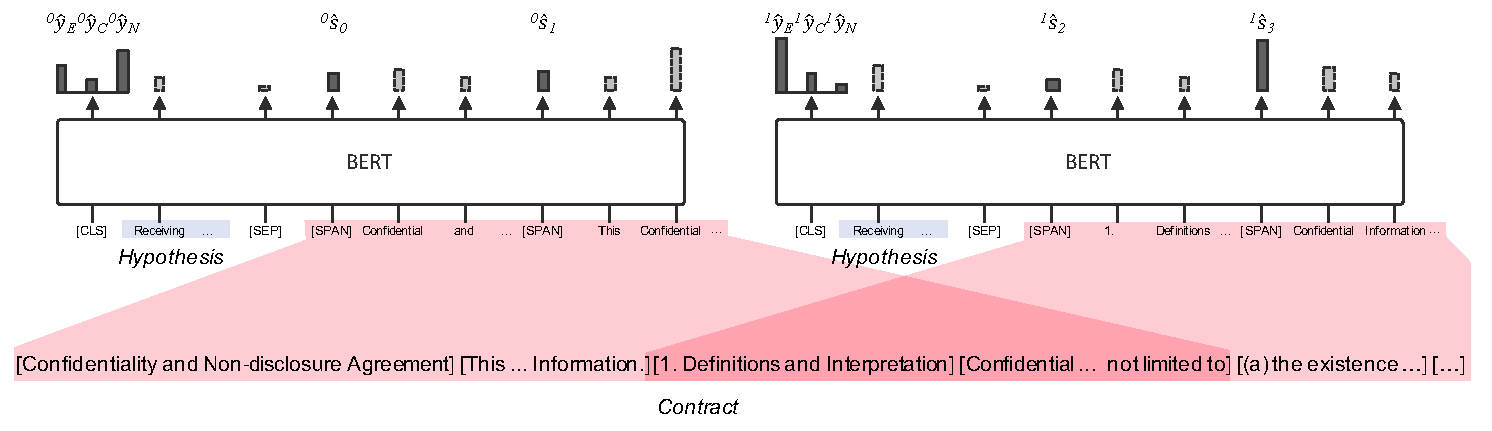
\includegraphics[width=\textwidth]{fig/model}
    \caption{Model architecture of proposed Span NLI BERT}\label{fig:model}
\end{figure*}

Transformer-based models have become a dominant approach for many NLP tasks.
Previous works implemented span identification on the Transformer architecture by predicting start and end tokens, scaling it to a document by splitting the document into multiple contexts with a static window and a stride size \cite{devlin_bert_2019,hendrycks_cuad_2021}.
The start/end token prediction makes the problem unnecessarily difficult because the model has to solve span boundary detection and evidence identification concurrently, whereas the definition of spans is usually fixed for many applications.
Splitting a document can be problematic when a span is split into multiple contexts or when a span does not receive enough surrounding context.

To that end, we introduce Span NLI BERT, a multi-task Transformer model that can jointly solve NLI and evidence identification, as well as addressing the above shortcomings of the previous works (\cref{fig:model}).
Instead of predicting start and end tokens, we propose to insert special \texttt{[SPAN]} tokens each of which represents a span consisting of subsequent tokens, and model the problem as straightforward multi-label binary classification over the \texttt{[SPAN]} tokens.
We also propose to split documents with dynamic stride sizes such that there exists at least one context setting for each span in which the span is not split and receives enough context.

\begin{Ualgorithm}[t]
    \fontsize{8pt}{10pt}\selectfont
    \SetAlgoLined
    \KwIn{Span boundary token indices $B = [b_0, b_1, ...]$, Tokens $T = [t_0, t_1, ...]$, min. \# of surrounding tokens $n$, max. context length $l$}
    \KwOut{List of overlapping contexts}
    $\text{contexts} = []$ \;
    $\text{start} = 0$ \;
    \While{$\text{len}(B)$ > 0}{
        \For{$b_i$ in $B$ where $b_i - \text{start} <= l$}{
            $B$.remove($b_{i-1}$) \;
            $\text{end} = b_{i-1}$ \;
        }
        contexts.append($T[\text{start}:(\text{start} + l)]$) \;
        $\text{start} = \text{end} - \text{n}$ \;
    }
    \Return contexts \;
    \caption{Dynamic context segmentation}\label{alg:dynamic_context_segmentation}
\end{Ualgorithm}

First, we split each document into contexts using \cref{alg:dynamic_context_segmentation}.
Given a user-specified maximum context length $l$ and a minimum number of surrounding tokens $n$, the algorithm adds first $l$ tokens to a context and marks the spans whose tokens have all been added to the context.
For the next context, it will start again from $n$ tokens before the next unmarked span and repeat this until all the spans are marked.
We mark variables associated with $m$-th context with a left superscript $m$ where necessary.

For each context, contract tokens and hypothesis tokens are concatenated with a \texttt{[SEP]} token and fed into a Transformer-based model.
For evidence identification, we place a randomly initialized multi-layer perceptron (MLP) on top of each \texttt{[SPAN]} token followed by sigmoid activation to predict a span probability $\hat{s}_i  \in \mathbb{R}$.
Likewise for NLI, we place a randomly initialized MLP on top of the \texttt{[CLS]} token followed by a softmax layer to predict \textsc{Entailment},  \textsc{Contradiction} and \textsc{NotMentioned} probabilities ${}^m\hat{y}_E, {}^m\hat{y}_C, {}^m\hat{y}_N \in \mathbb{R}$, respectively.

For evidence identification loss $\ell_{span}$ of a single context, we employ cross entropy loss between the predicted span probability $\hat{s}_i$ and the ground truth span label $s_i \in \{0, 1\}$.
\begin{equation}
    \ell_{span} = \sum_i \left(- s_i \log \hat{s}_i - (1 - s_i) \log (1 - \hat{s}_i )\right)
\end{equation}
Although there exists no evidence span when NLI label is \textsc{NotMentioned}, we nevertheless incorporate such an example in the evidence identification loss with negative span labels $s_i = 0$.

For NLI loss $\ell_{NLI}$, we likewise employ cross entropy loss between the predicted NLI probabilities $\hat{y}_E, \hat{y}_C, \hat{y}_N$ and the ground truth span labels $y_E, y_C, y_N \in \{0, 1\}$.
However, there are contexts without an evidence span despite the NLI label being \textsc{Entailment} or \textsc{Contradiction}.
This causes inconsistency between what the model sees and its teacher signal.
Thus, we ignore the NLI predictions for the contexts that do not contain an evidence span.
\begin{equation}
    \ell_{NLI} = \begin{cases}
        - \sum_{L\in\{E, C ,N\}} y_L \log \hat{y}_L, & \text{if } {}^\exists s_i = 1, \\
        0, & \text{otherwise}.
    \end{cases}
\end{equation}
The multitask loss $\ell$ for a single context is then
\begin{equation}
    \ell = \ell_{span} + \lambda \ell_{NLI},
\end{equation}
where $\lambda$ is a hyperparameter that controls the balance between the two losses.
We mix contexts from different documents during training, thus contexts from a single document may appear in different mini batches.

Since each document is predicted as multiple contexts, results from these contexts have to be aggregated to obtain a single output for a document.
For the evidence identification, we simply take the average of span probabilities over different model outputs.
\begin{equation}
    {}^\ast\hat{s}_i = \frac{1}{M_i} \sum_m {}^m\hat{s}_i,
\end{equation}
where $M_i$ is the number of contexts that have the full $i$-th span in its context.

For NLI, we weighted the NLI probabilities by the sum of the span probabilities:
\begin{equation}
    {}^\ast\hat{y}_\bullet =  \frac{1}{\sum_m \frac{1}{S_m} \sum_i {}^m\hat{s}_i}\sum_m \left({}^m\hat{y}_\bullet \cdot \frac{1}{S_m} \sum_i {}^m\hat{s}_i\right),
\end{equation}
where $S_m$ is the number of \texttt{[SPAN]} tokens in the $m$-th context.
This is based on an intuition that contexts with evidence spans should contribute more to NLI.
